La struttura delle pagine interne al sito è molto eterogenea, fattore che crea confusione e disorientamento da parte dell'utente. Infatti i layout possibili per le pagine interne (le hanno lo stesso livello di annidamento o addirittura appartengono allo stesso menù) individuati sono 3:
	\begin{itemize}
		\item Il primo, comune a tutte le voci del menù di sinistra (tranne la voce "biblioteca") e alle voci del menù in alto a destra:
\begin{center}
\begin{figure}[h!]
           \begin{center}
           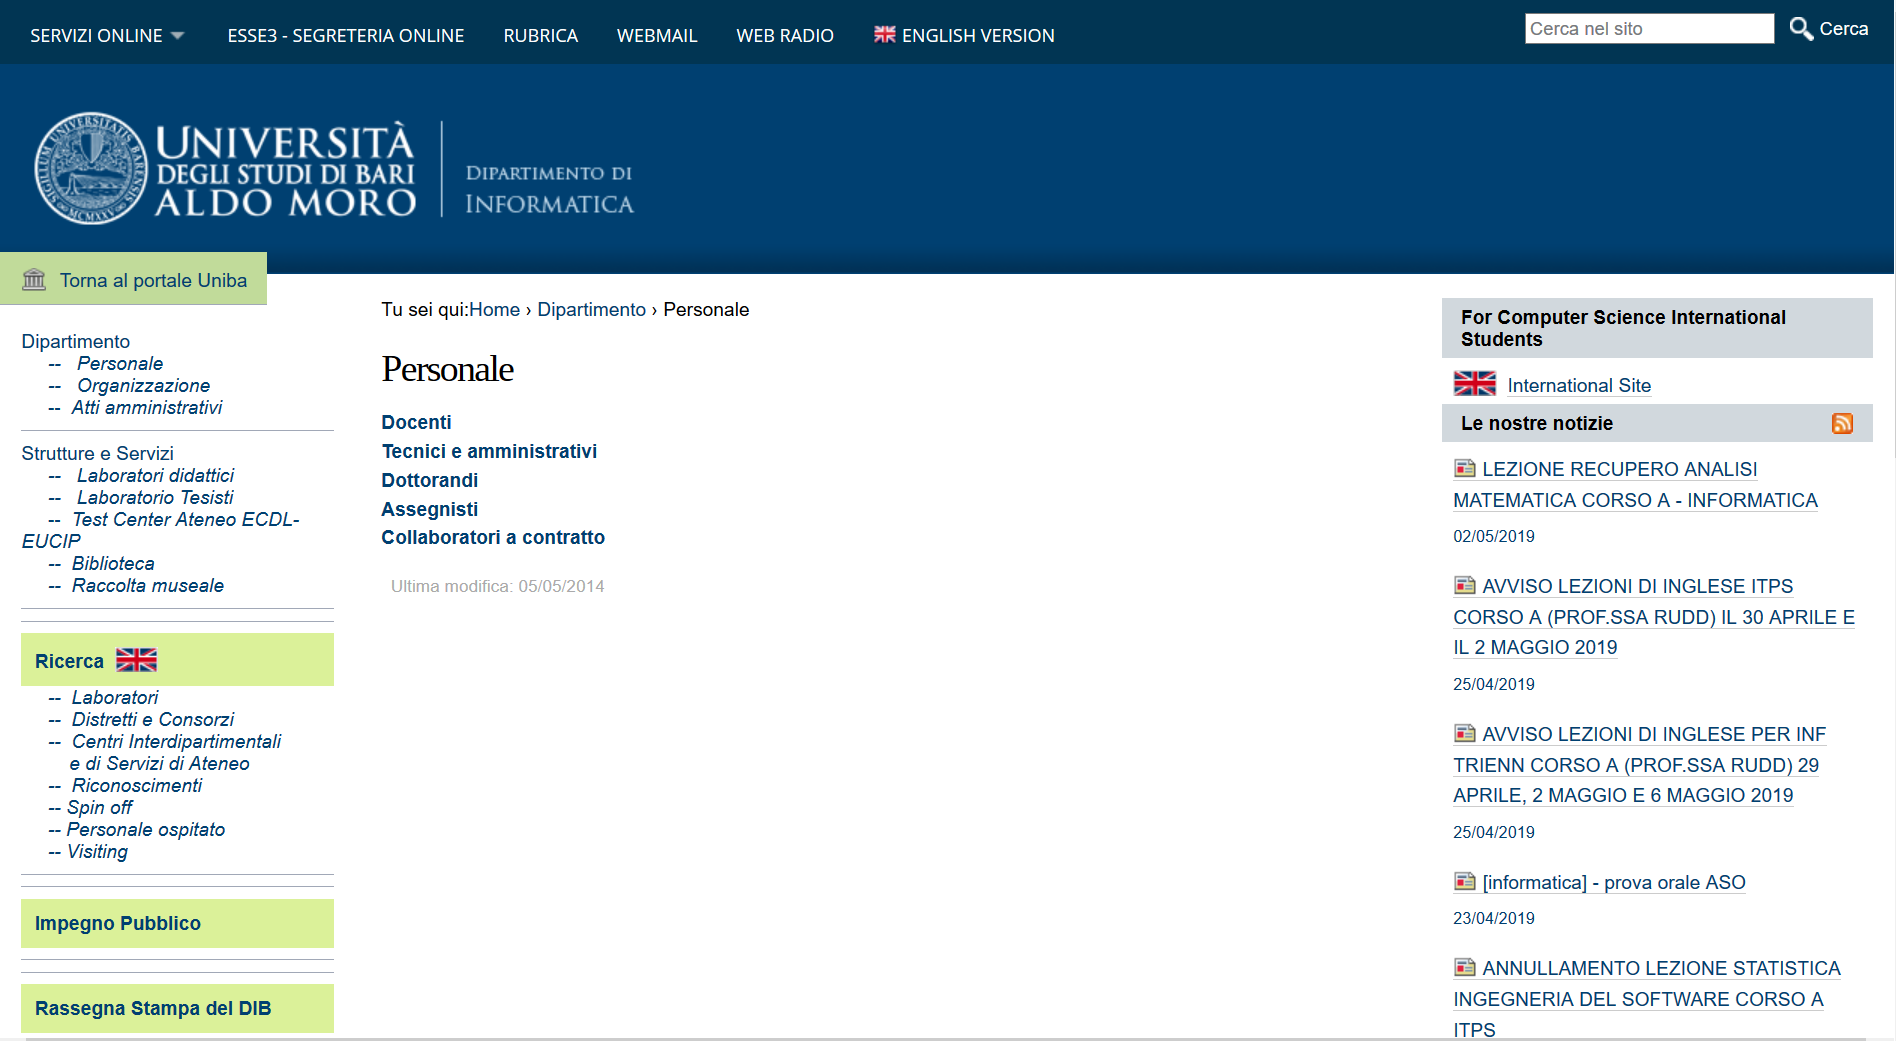
\includegraphics[scale=0.40]{C:/Users/elepo/Desktop/UNI/WIM/ANALISI_SITO/Relazione/sez/Pag_interne/layout1.png}
           \caption{Layout 1}
           \end{center}
  \end{figure}
\end{center}
		\item Un secondo layout, completamente incongruente rispetto al primo, proprio solo della voce "biblioteca" del menù di sinistra, che reindirizza al sito dell'ateneo Aldo Moro:
		\begin{center}
\begin{figure}[h!]
           \begin{center}
           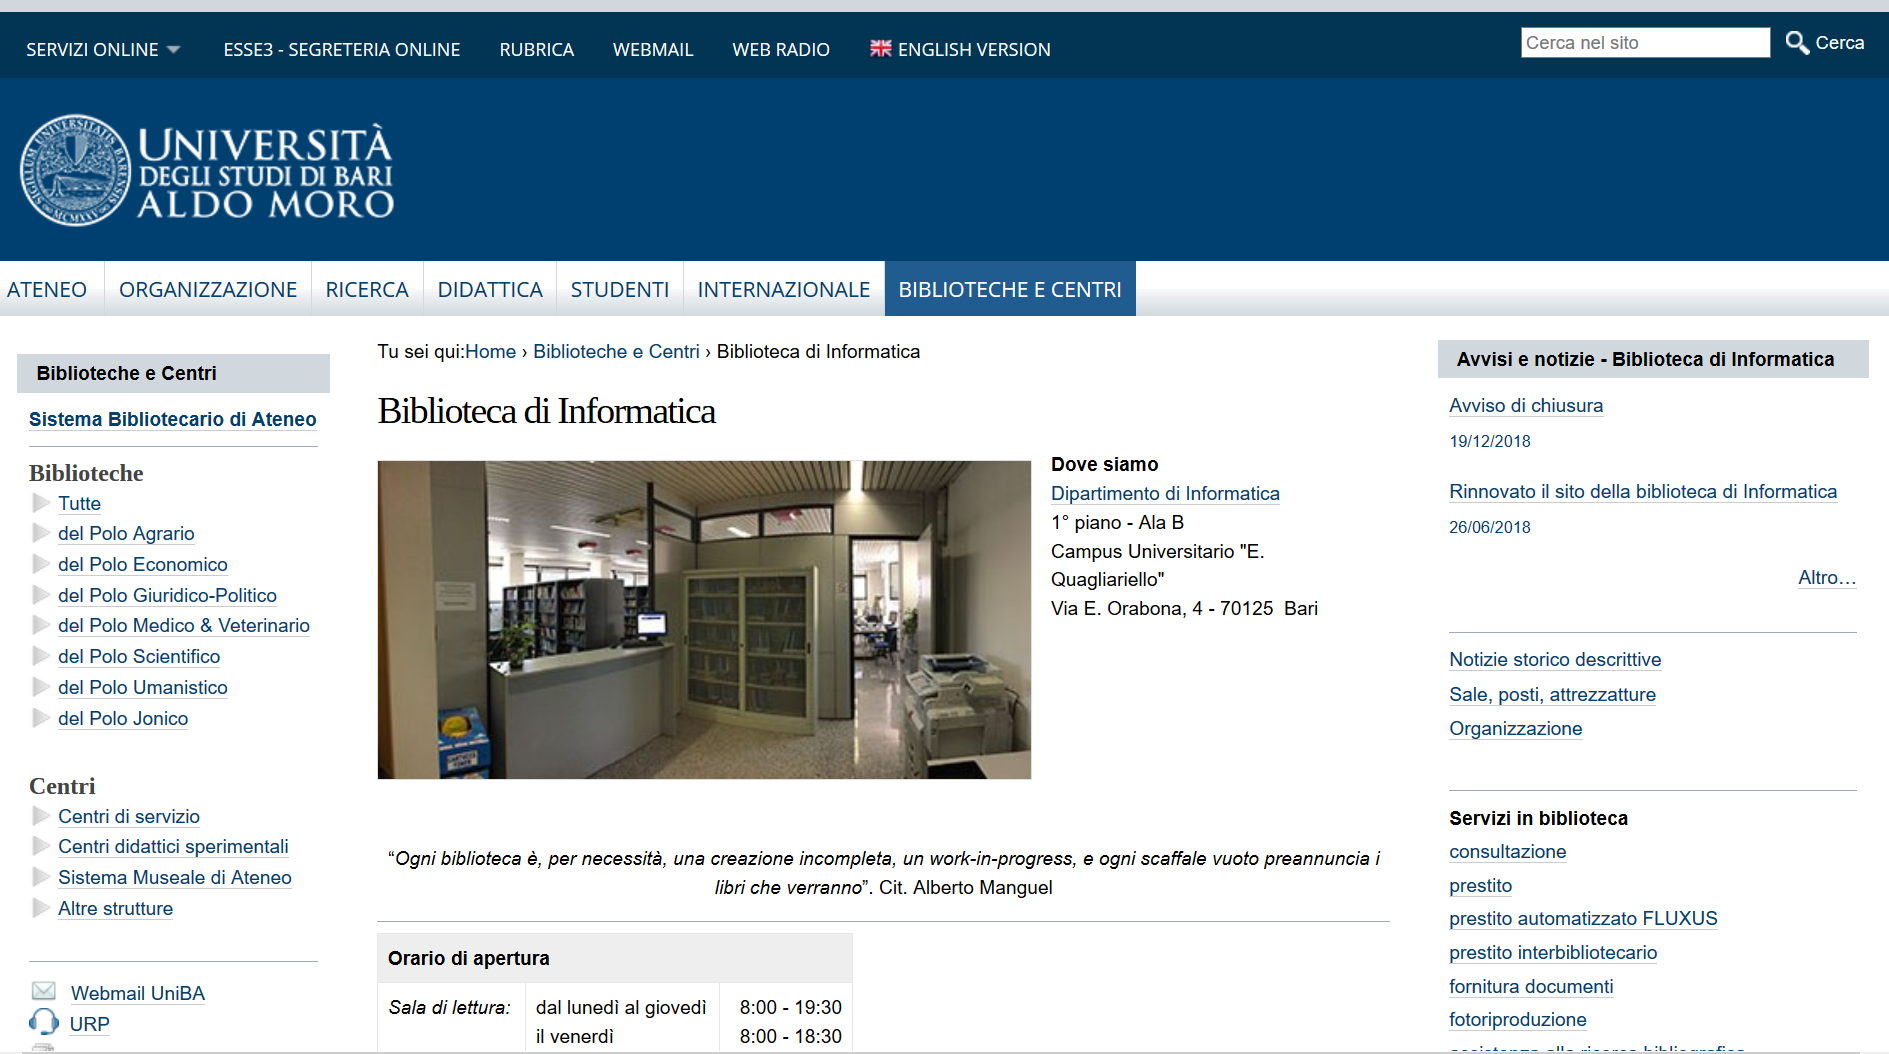
\includegraphics[scale=0.40]{C:/Users/elepo/Desktop/UNI/WIM/ANALISI_SITO/Relazione/sez/Pag_interne/layout2.png}
           \caption{Layout 2}
           \end{center}
  \end{figure}
\end{center}
\newpage
		\item Un terzo layout comune alle voci del menù di destra in basso:
		\begin{center}
\begin{figure}[h!]
           \begin{center}
           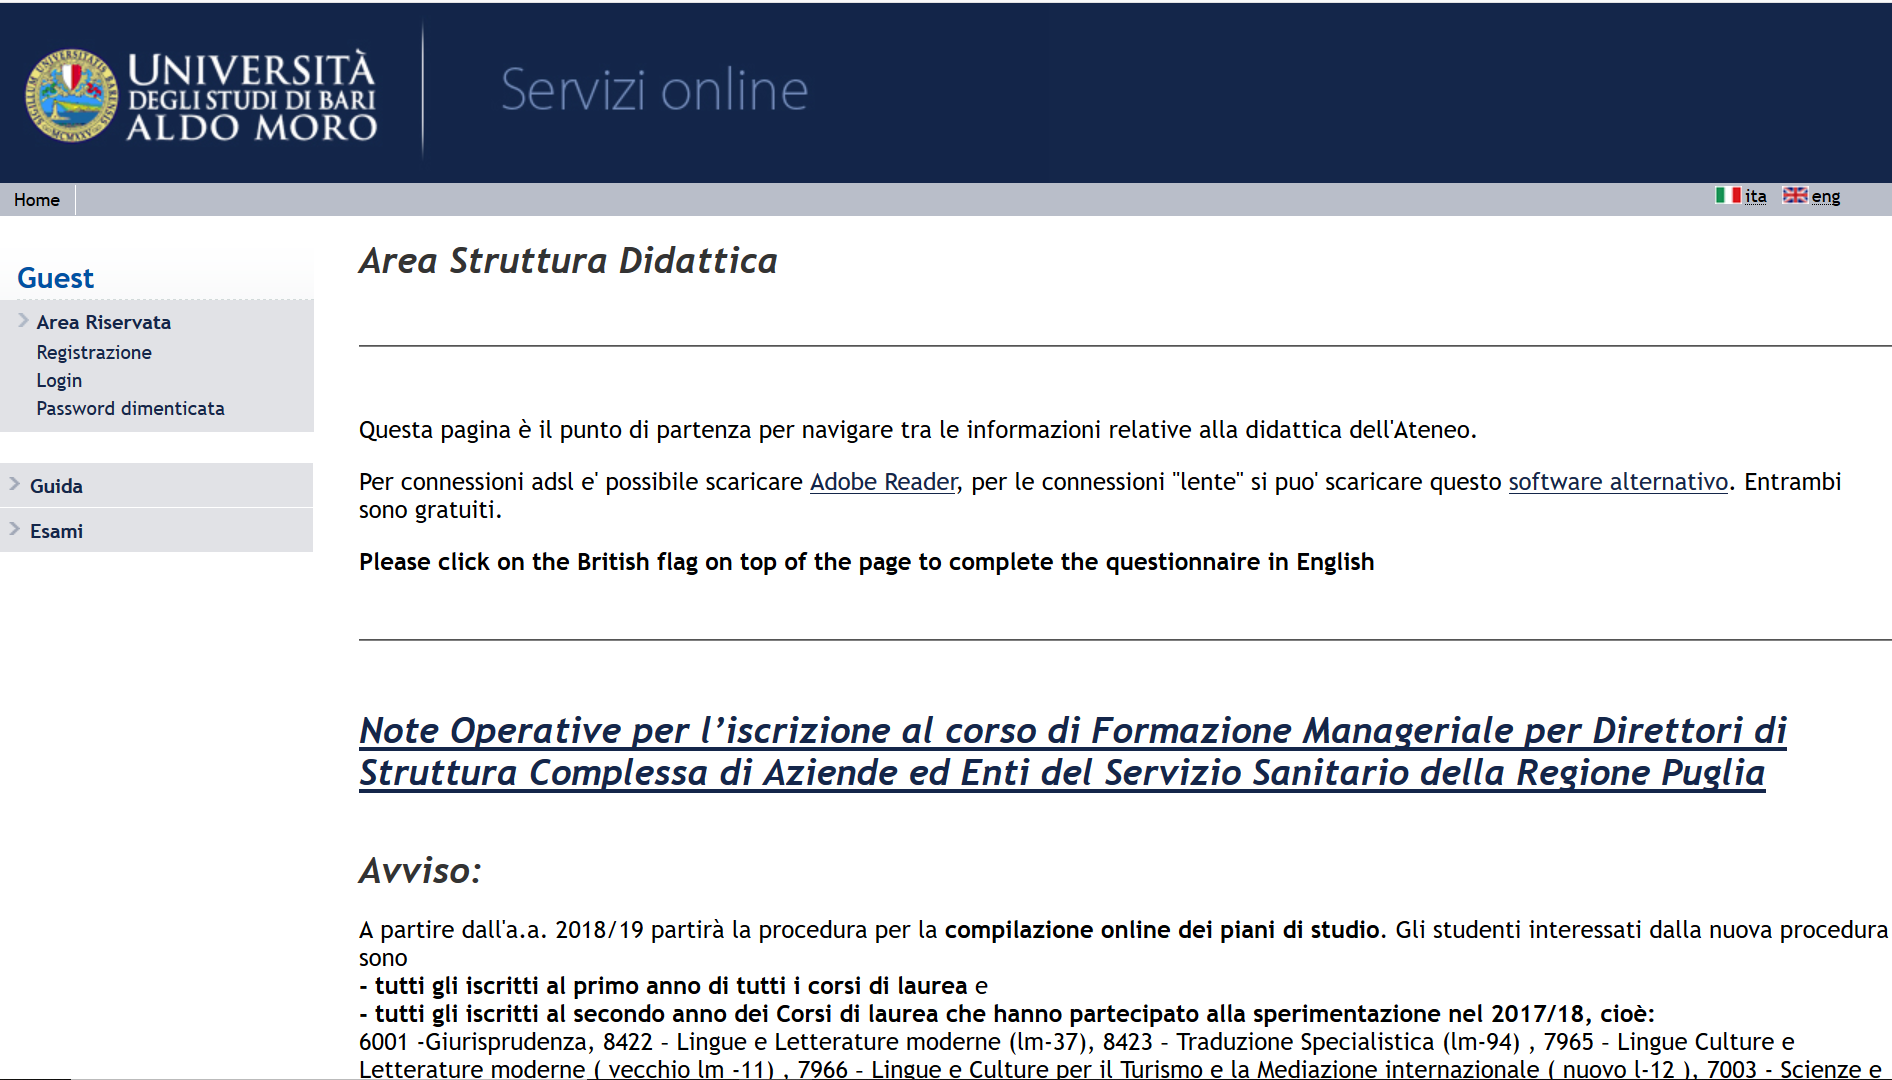
\includegraphics[scale=0.40]{C:/Users/elepo/Desktop/UNI/WIM/ANALISI_SITO/Relazione/sez/Pag_interne/layout3.png}
           \caption{Layout 3}
           \end{center}
  \end{figure}
\end{center}
	\end{itemize}
A mio avviso il fatto che una voce del menù di sinistra ("biblioteca") abbia un layout completamente differente rispetto alle voci appartenenti allo stesso menù è molto disorientante, dal momento che voce appartenenti allo stesso menù o a livelli di annidamenti analoghi dovrebbero avere lo stesso layout.\\
Un altro fattore negativo è l'utilizzo inconsistente del breadcrumb: per esempio per voci allo stesso livello di annidamento troviamo due breadcrumb totalmente differenti:
